
\begin{theorem}{Potenzreihen}
	Sei $\sum_{k=0}^\infty c_k x^k$ eine Potenzreihe mit positiven Konvergenzradius $\rho > 0$. Dann ist $f(x) = \sum_{k=0}^\infty c_k (x-x_0)^k$ auf $ ]x_0 - \rho, x_0 + \rho[$ differenzierbar und $f'(x) = \sum_{k=1}^\infty k c_k (x - x_0) ^{k-1}$ für alle $x \in ]x_0 - \rho, x_0 + \rho[$.
\end{theorem}

\begin{theorem}{Taylorreihen}
	Sei $f : [a,b] \to \R$ stetig und in $ ]a,b[$ $(n+1)$-mal differenzierbar.
	Für jedes $a < x \leq b$ gibt es $\xi \in ]a,x[$ mit\\
	$f(x) = \sum_{k=0}^n \frac{f^{(k)} (a)}{k!} (x - a)^k + \frac{f^{(n+1)} (\xi)}{(n+1)!} (x - a)^{n+1}$.
\end{theorem}
\noindent Jede glatte Funktion kann als Potenzreihe angenähert werden, dafür brauchen wir ein sogenanntes Taylor-Polynom (oder Taylorreihen). Die trigonometrischen Funktionen sind genau solche Taylorreihen.
\begin{corollary}{Bekannte Taylorreihen}\\
    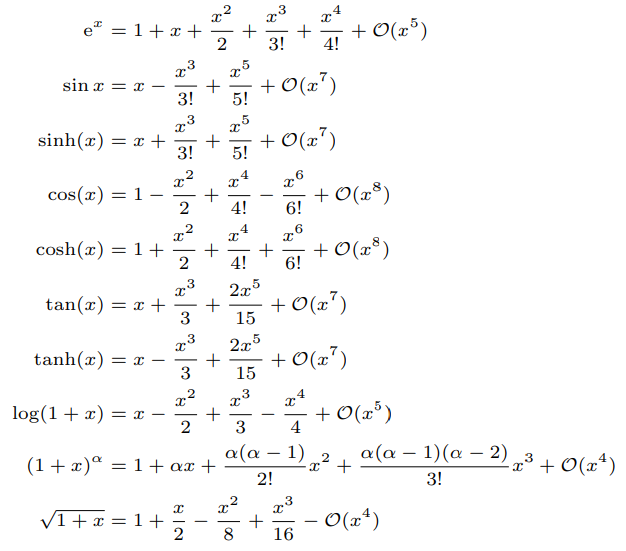
\includegraphics[scale=0.5]{Analysis1/zsf/Images/Differential/bekannte_taylorreihen.png}
\end{corollary}
\subsubsection{Konvergenz mit Taylorreihen}
                    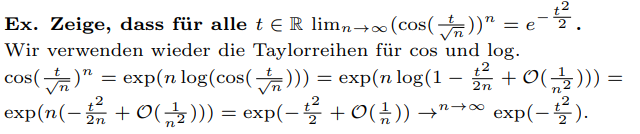
\includegraphics[scale=0.5]{Analysis1/zsf/Exercises_Images/folgen_reihen/5.png}
                    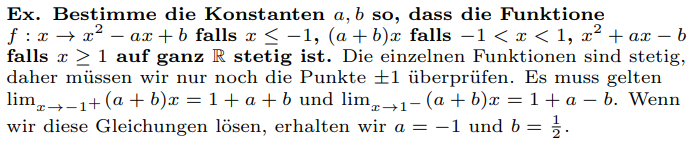
\includegraphics[scale=0.5]{Analysis1/zsf/Exercises_Images/folgen_reihen/4.png}
\raggedcolumns
\columnbreak
\begin{theorem}[important]{Taylor Approximation}
	Sei $f: [c,d] \to \R$ stetig und in $ ]c,d[$ $(n+1)$-mal differenzierbar.
	Sei $c<a<d$.
	Für alle $x \in [c,d]$ gibt es $\xi$ zwischen $x$ und $a$, sodass
	\begin{equation*}
		f(x) = \sum_{k=0}^n \frac{f^{(k)} (a)}{k!} (x - a)^k + \frac{f^{(n+1)} (\xi)}{(n+1)!} (x - a)^{n+1}
	\end{equation*}
\end{theorem}
\noindent  Der letzte Term $\frac{f^{(n+1)} (\xi)}{(n+1)!} (x - a)^{n+1}$ wird meist zur Fehlerabschätzung innerhalb eines Bereiches von a verwendet. Man nimmt daher den Wert von $\xi \in ]a, x[$, so dass der Fehlerterm am grössten ist.




